\label{app:ferrProp}
There are a number of ferrites used for the damping of cavity modes in accelerator equipment, some of the details of which are given here. For the use of ferrite as a damping material, the important material properties to consider are the complex permeability $\mu_{r} = \mu^{'} - j\mu^{"}$, which determines the degree of damping of cavity modes, and the Curie temperature $T_{c}$ which determines to which temperature the ferrite will remain effective as a damping material to, important due to the significant power loss that may occur in the ferrite. Here we give examples of 3 ferrites commonly used for damping of cavity modes, and one additional ferrite that shows promise for use due to a high Curie temperature.

An additional figure of merit is the penetration depth of the ferrite. This figure determines how far the magnetic field penetrates into the ferrite, thus giving a guide as to how much ferrite is necessary to effectively damp any cavity modes. This is a frequency dependent value, given by

\begin{equation}
\delta\left( f \right) = \frac{c}{2\pi f}\frac{1}{\Re{}e\left[\sqrt{1-\epsilon_{r}\left( f \right) \mu_{r}\left( f \right)}\right]}.
\end{equation}

\section{TT2-111R}

TT2-111R is a ferrite made by Transtech. It is a variant of the TT2-111 ferrite with a slight conductivity to reduce the build up of electrostatic charge. TT2-111R is useful in as it has a very high Curie temperature $T_{c}\approx 375^{\circ}C$. Some material properties are shown in Tab.~\ref{tab:tt2111rProp}. The complex permeability is shown in Fig.~\ref{fig:tt2111rPerm} and the penetration depth in Fig.~\ref{fig:tt2111rPenDepth}.

\begin{table}
\caption{A selection of the physical properties of TT2-111R}
\label{tab:tt2111rProp}
\begin{center}
\begin{tabular}{c | c | c}
$\epsilon^{'}$ & 12.5 & \\ \hline
Conductivity  & 10$^{-1}$ & S m$^{-1}$\\ \hline
$T_{c}$ & 375 & $^{\circ c}$C \\
\end{tabular}
\end{center}
\end{table}

\begin{figure}
\subfigure[]{
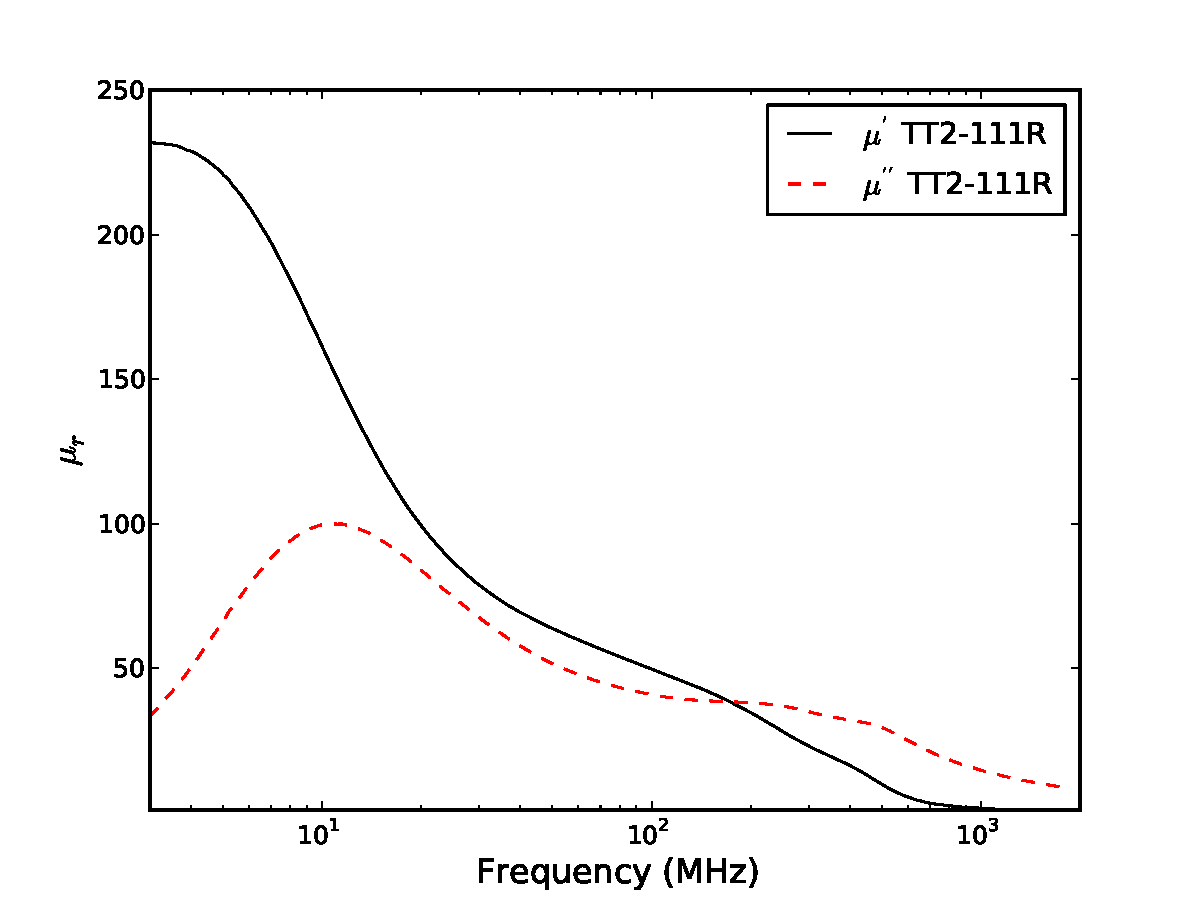
\includegraphics[width=0.5\textwidth]{appendices/figures/tt2111rPerm.pdf}
\label{fig:tt2111rPerm}
}
\subfigure[]{
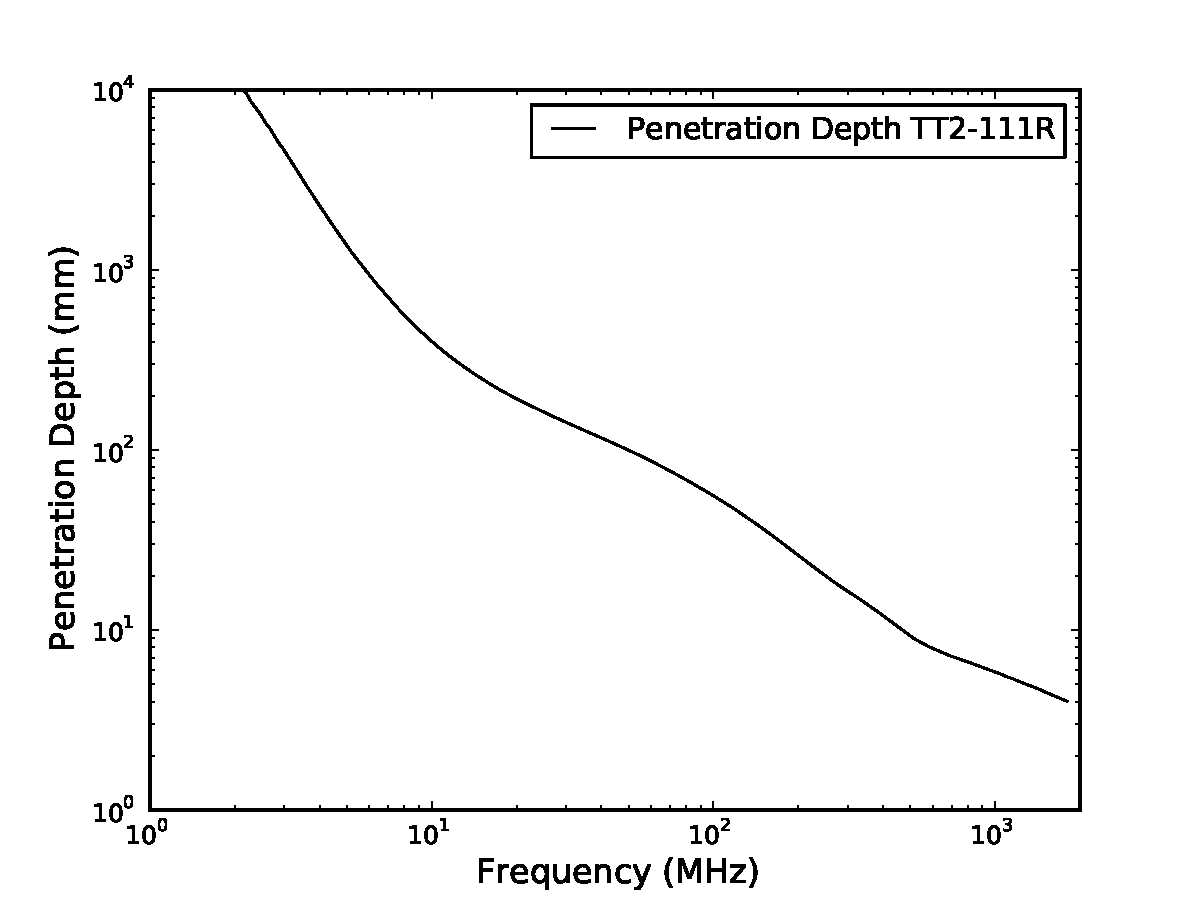
\includegraphics[width=0.5\textwidth]{appendices/figures/tt2111rPenDepth.pdf}
\label{fig:tt2111rPenDepth}
}
\caption{The permeability \subref{fig:tt2111rPerm} and penetration depth \subref{fig:tt2111rPenDepth} for TT2-111R.}
\end{figure}

\section{4S60}

4S60 is a ferrite made by Ferroxcube. It has a slight conductivity. Some material properties are shown in Tab.~\ref{tab:4s60Prop}. The complex permeability is shown in Fig.~\ref{fig:4s60Perm} and the penetration depth in Fig.~\ref{fig:4s60PenDepth}.

\begin{table}
\caption{A selection of the physical properties of 4S60}
\label{tab:4s60Prop}
\begin{center}
\begin{tabular}{c | c | c}
$\epsilon^{'}$ & 10 & \\ \hline
Conductivity  & 10$^{-5}$ & S m$^{-1}$\\ \hline
$T_{c}$ & 100 & $^{\circ c}$C \\
\end{tabular}
\end{center}
\end{table}

\begin{figure}
\subfigure[]{
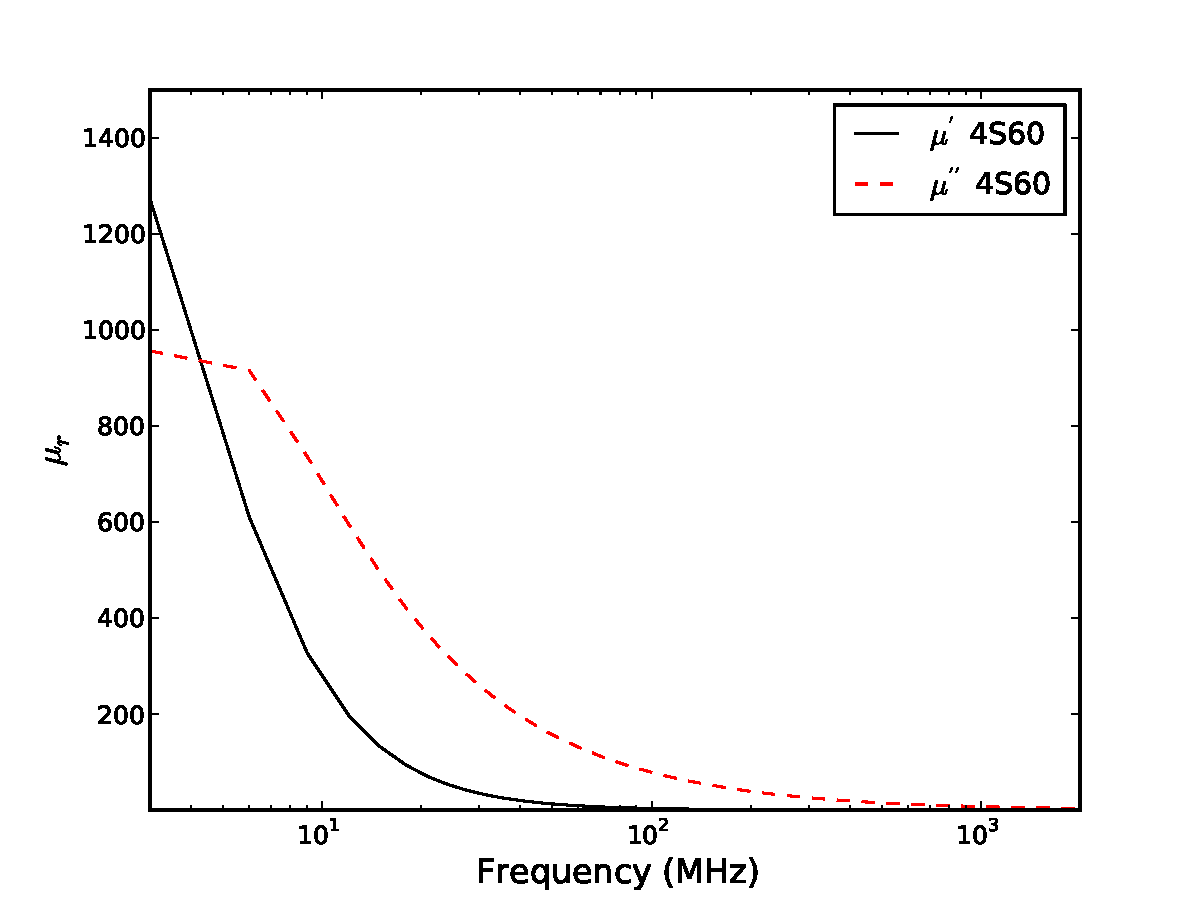
\includegraphics[width=0.5\textwidth]{appendices/figures/4s60Perm.pdf}
\label{fig:4s60Perm}
}
\subfigure[]{
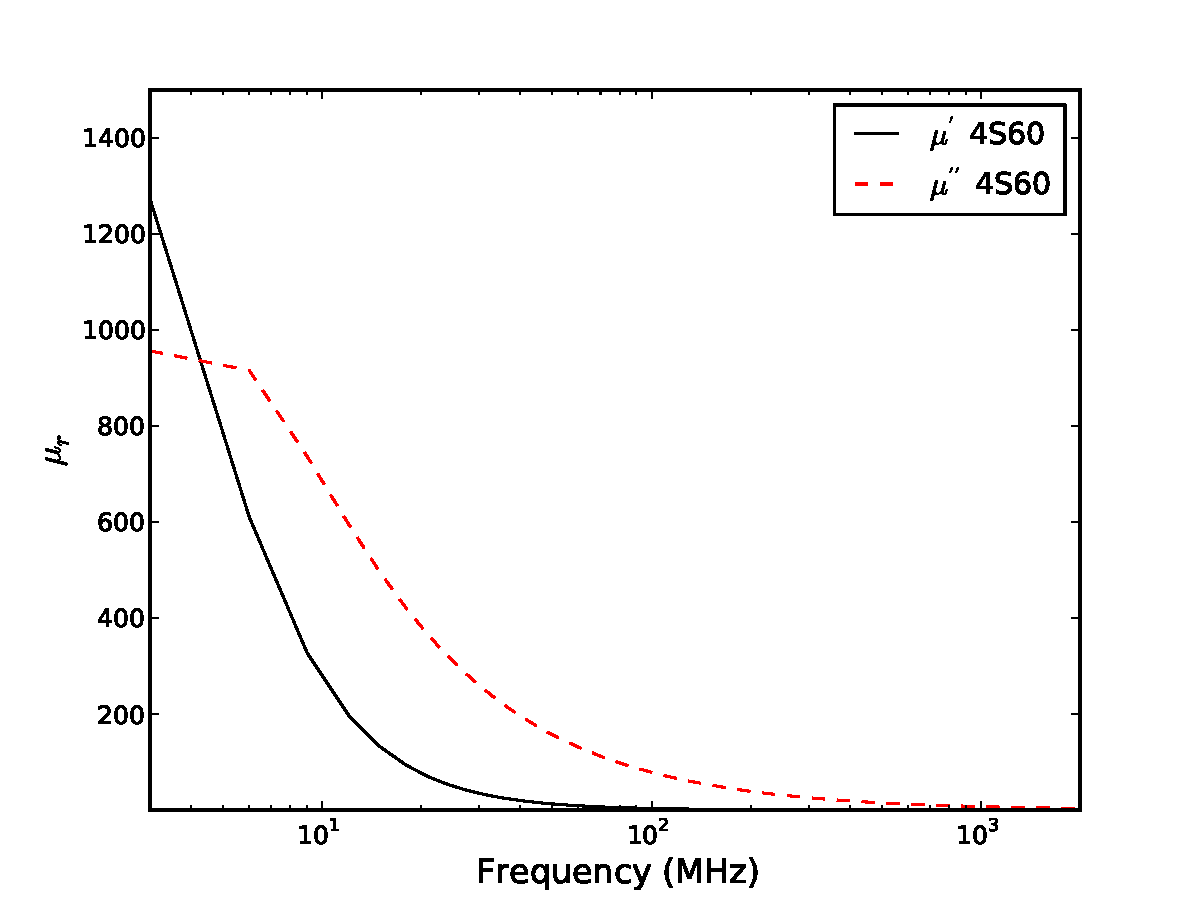
\includegraphics[width=0.5\textwidth]{appendices/figures/4s60PenDepth.pdf}
\label{fig:4s60PenDepth}
}
\caption{The permeability \subref{fig:4s60Perm} and penetration depth \subref{fig:4s60PenDepth} for 4S60.}
\end{figure}

\section{4A4}

4A4 is a ferrite made by Transtech. It has a mild conductivity to reduce electrostatic buildup, and is typically used as a ferrite in fast pulsed kicker magnets due to it's beneficial properties. It is commonly used to damp cavity modes due to it's good vacuum performance. Some material properties are shown in Tab.~\ref{tab:4a4Prop}. The complex permeability is shown in Fig.~\ref{fig:4a4Perm} and the penetration depth in Fig.~\ref{fig:4a4PenDepth}.


\begin{table}
\caption{A selection of the physical properties of 4A4}
\label{tab:4a4Prop}
\begin{center}
\begin{tabular}{c | c | c}
$\epsilon^{'}$ & 10 & \\ \hline
Conductivity  & 10$^{-6}$ & S m$^{-1}$\\ \hline
$T_{c}$ & 375 & $^{\circ c}$C \\
\end{tabular}
\end{center}
\end{table}

\begin{figure}
\subfigure[]{
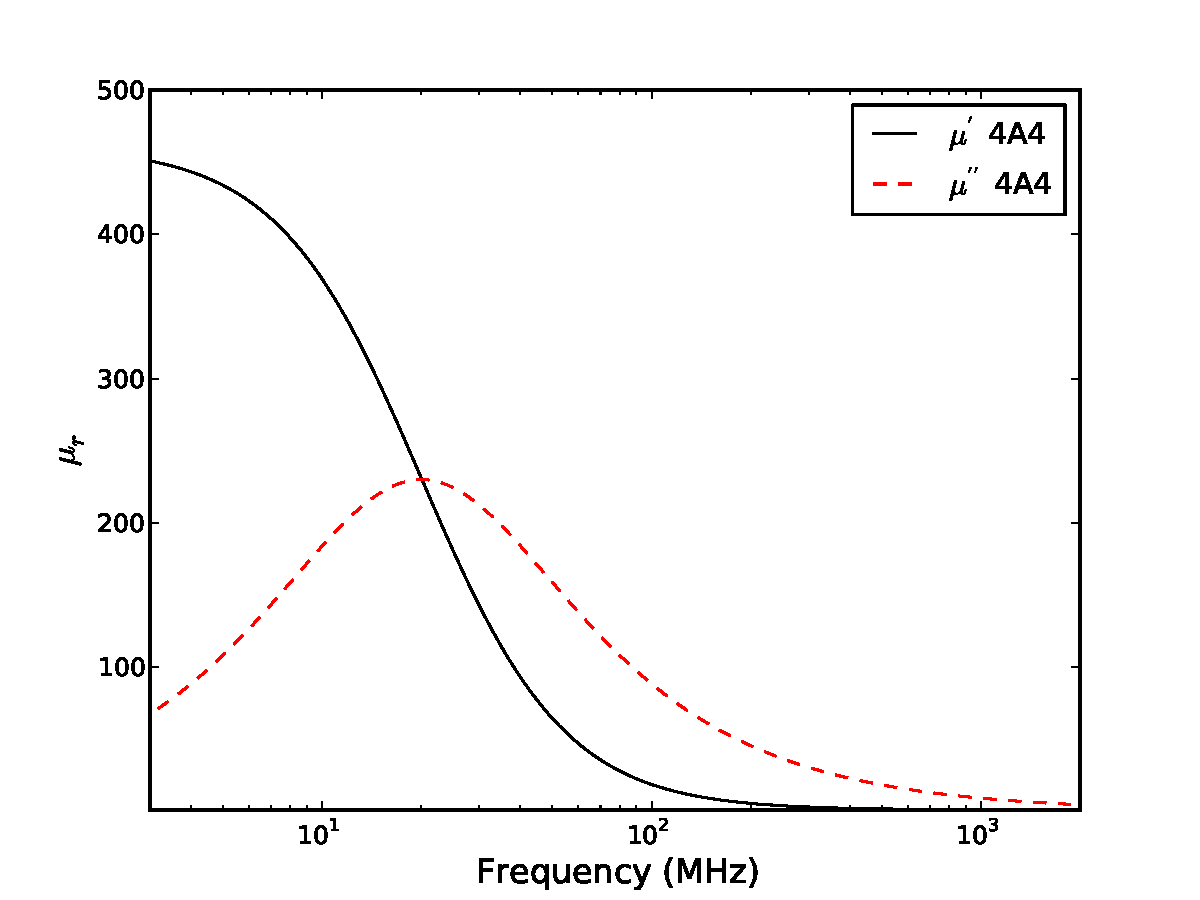
\includegraphics[width=0.5\textwidth]{appendices/figures/4a4Perm.pdf}
\label{fig:4a4Perm}
}
\subfigure[]{
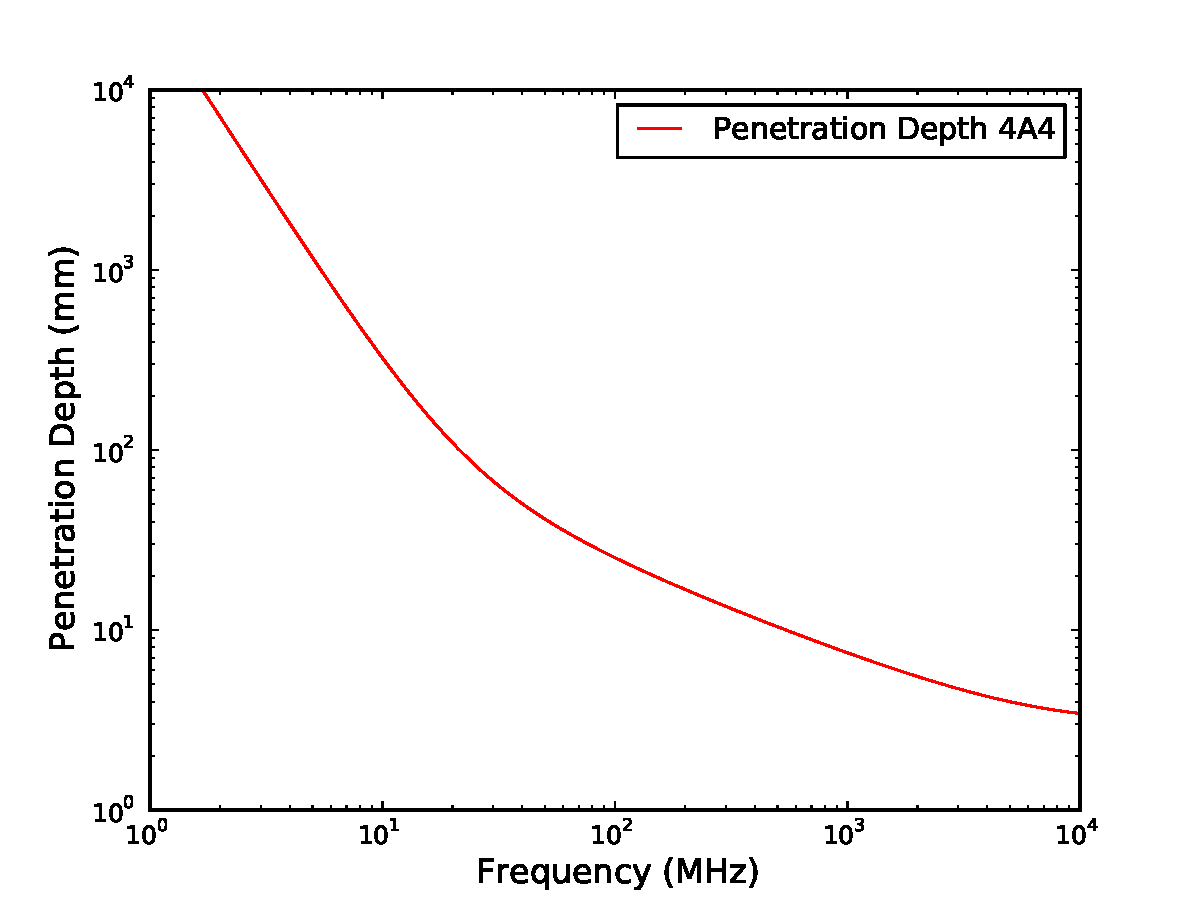
\includegraphics[width=0.5\textwidth]{appendices/figures/4a4PenDepth.pdf}
\label{fig:4a4PenDepth}
}
\caption{The permeability \subref{fig:4a4Perm} and penetration depth \subref{fig:4a4PenDepth} for 4A4.}
\end{figure}